\chapter{Review of my favorite transients: Gamma Ray Bursts}
\label{grb}

\section{Introduction}

\gls{grbs} are the most luminous transient events in the observed Universe. When they occur, they outshine an entire galaxy \cite{Meszaros,MBthesis}. 
Gamma-ray luminosities of \gls{grbs} are of the order $10^{52} \, \mathrm{erg \, s^{-1}}$ which can be compared to the $10^{33} \, \mathrm{erg \, s^{-1}}$ emitted by our Sun, $10^{41} \, \mathrm{erg \, s^{-1}}$ by a supernova and $10^{45} \, \mathrm{erg \, s^{-1}}$ by a whole galaxy. 

First discovered in 1967 by the Vela satellites flown by the U.S. Department of Defense, \gls{grbs} continue to intrigue and puzzle scientists to this day.
However, research in the past decades have revealed much about them including that they are extragalactic in origin, isotropically distributed and that they come in at least two populations.

\gls{grbs} are classified as {\bf long} if they last for $t_{GRB} > 2 \, \mathrm{s}$ and {\bf short} if they last for $t_{GRB} < 2 \, \mathrm{s}$. Long bursts are associated with the collapse of massive stars or hypernovae and short bursts are associated with mergers of binaries composed of neutron star-neutron star or neutron star-black hole \cite{Meszaros}. 

In August of 2017, for the first time in history, multimessenger observation of a short \gls{grb} was performed by the LIGO, Virgo and Fermi collaborations, confirming the association of short \gls{grbs} with a binary neutron star merger~\cite{ligo_short}. This marked the first observation of a messenger other than photons from a \gls{grb}. Indeed, no other messengers or particles have been known to come from \gls{grbs}, although theories predict that \gls{grbs} are environments where particles could get accelerated to the highest energies.

The detection of \gls{grb} {\bf neutrinos} would provide unambiguous proof for hadronic acceleration in these cosmic explosions and could also explain the origin of the cosmic ray flux at ultra-high energies.
From gamma-ray observations alone, theorists have hypothesized that regardless of the nature of the underlying source or progenitor, \gls{grbs} are produced by the dissipation of the kinetic energy of a relativistically expanding fireball. Protons may be Fermi accelerated in this dissipation region to energies $> 10^{20} \, \mathrm{eV}$. Interactions between fireball gamma-ray photons of energy $\sim 1 \, \mathrm{MeV}$ and accelerated protons of energy $\sim 10^{15} \, \mathrm{eV}$ could lead to photo-meson production of pions which upon decaying would result in an accompanying burst of $\sim 10^{14} \, \mathrm{eV}$ neutrinos (Waxman \textit{et al.} \cite{Waxmanreview,firstcalc}). 


\subsection{GRB emission}

\gls{grbs} are characterized by a two-part emission: {\bf prompt} and {\bf afterglow}. Gamma-rays are emitted during the prompt emission period followed by softer and softer photons such as X-rays, UV rays, and so on during the afterglow emission period. As discussed in  Section~\ref{early_theory}, neutrinos are predicted from \gls{grbs} following an opposite spectrum to that of photons, in other words, harder and harder energy neutrinos with time. The type of emissions from a \gls{grb} is summarized in Figure~\ref{grb_emission}. 

\begin{figure}
\centering
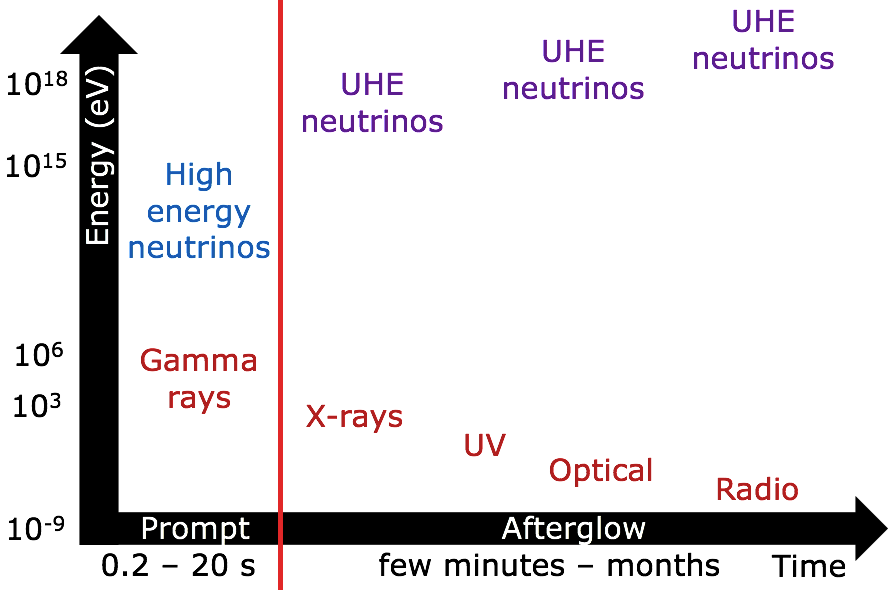
\includegraphics[width=1.0\textwidth]{figures/grb_emission.png}
\caption{Illustration of the predicted emission from \gls{grbs}. Note that GRBs are extremely diverse. Most importantly, note that UHE neutrinos are more likely to be produced during the afterglow of a GRB, as opposed to during its prompt emission.}
\label{grb_emission}
\end{figure}

As can be seen in Figure~\ref{grb_emission}, \gls{grbs} are extremely diverse. The prompt emission is typically between 0.2 and 20 seconds long. Note that the prompt emission can, occasionally, last for several hundreds of seconds as was seen in the case of a 5400 second long \gls{grb} that was reported in \cite{longhardgrb}. The afterglow emission time period for \gls{grbs} is even more diverse. The afterglows can last from anywhere between few minutes to several months. Swift scientist at the Mullard Space Science Laboratory, Mat Page, showed me the flux vs. time plot of a \gls{grb} with afterglow observations in X-ray that continued for over a year! 
%A plot from his talk showing this is presented in Figure~\ref{long_afterglow}. 
Mat shared that eventually the observers 
decided to move on and assign observation time to other objects.

Afterglow records might not be available for a few other reasons. 
Sometimes, afterglows are not observed at all as no telescope is pointing at the object for follow-up in afterglow. So, the absence of a record for an afterglow does not necessarily mean that there was no afterglow. Moreover, afterglow photons can get absorbed by dust and not be able to reach us. Thanks to my discussions with Swift observers at Mullard Space Science Laboratory for these insights.

%\begin{figure}
%\centering
%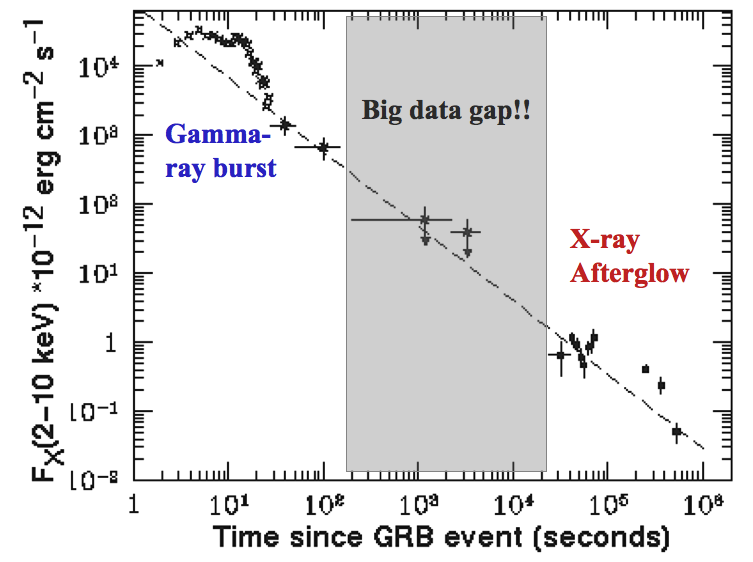
\includegraphics[width=1.0\textwidth]{figures/long_afterglow.png}
%\caption{Plot from a talk by Mat Page who is a Swift scientist based at Mullard Space Science Laboratory, United Kingdom. Observations of afterglow emission in X-ray were made for this GRB for over a year!}
%\label{long_afterglow}
%\end{figure}

%------------------------------------------------------------------------
%-----------------------NEW SECTION----------------------------
%------------------------------------------------------------------------

\section{GRB theory in the early days}
\label{early_theory}

The most widely accepted theory for \gls{grbs} endorses a relativistic fireball. 
The observation of gamma-rays (photons) guided this theory. In fact, the observed photon spectrum was the starting point for \gls{grb} theorists. Up until 1994, \gls{grbs} had been observed to emit photons in the energy range between a few keV and a few tens of MeV. In 1994, however, a very energetic burst was reported by \cite{longhardgrb} that emitted photons of energy up to 18 GeV. Other observations such as by the Fermi observatory \cite{fermishorthardgrb} have confirmed this hardness of the photon spectrum from \gls{grbs}. It was argued that since observed photons from the gamma-ray emitting region of the \gls{grb} do make it out to us, the optical depth in this region, $\tau_{\gamma \gamma}$ must be $< 1$. Now, the optical depth $\tau_{\gamma \gamma}$ is a function of the Lorentz factor $\Gamma$ (see review by Waxman \cite{Waxmanreview}) and thus from $\tau_{\gamma \gamma}$ it was obtained that the gamma-ray emitting region in a \gls{grb} must be moving with a Lorentz factor $\Gamma \geq 100$. Thus, the fireball model says that the gamma-ray emitting region of a \gls{grb} is relativistically expanding.

It was theorized that \gls{grbs} are produced by the dissipation of the kinetic energy of a relativistically expanding fireball. The expanding fireball has regions of over-density moving at different speeds. When these regions collide, shocks are produced. Particles are accelerated to relativistic speeds. The relativistic ejecta of a \gls{grb} may undergo internal collisions resulting in prompt emission as well as collisions with the interstellar medium resulting in afterglow emission. In these collisions, shock accelerated electrons emit synchrotron and inverse-Compton radiation in the form of gamma-rays. Thus, it was theorized that part of the kinetic energy of the \gls{grb} is the source of the observed gamma-radiation. It may be that the kinetic energy is converted to energy of electrons, energy in magnetic fields and energy of protons. A helpful review on these theories can be found in~\cite{Meszaros}.

No neutrinos are produced in the leptonic theory of \gls{grbs}. In the leptonic theory of \gls{grbs}, most of the kinetic energy of the \gls{grb} is assumed to go into energy of the electrons (leptons) and the electrons then emit gamma-radiation in the form of synchrotron and inverse-Compton radiation. There are no interacting baryons and no neutrinos produced in this picture. 

\begin{figure}
\centering
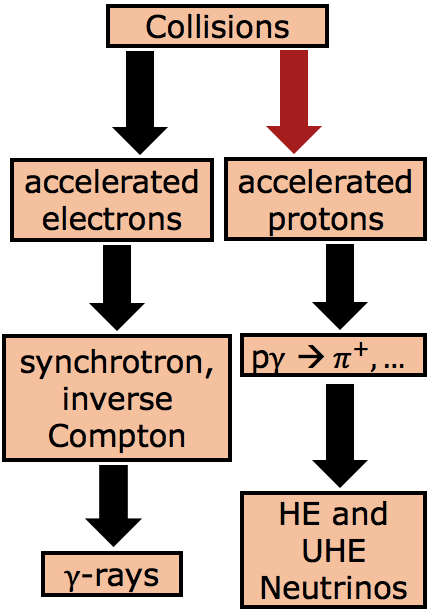
\includegraphics[width=0.8\textwidth]{figures/grb_hadronic.png}
\caption{Summary of the hadronic theory of \gls{grbs}. This theory predicts the production of high energy and ultra-high-energy neutrinos from \gls{grbs}.}
\label{grb_hadronic}
\end{figure}

\subsection{Neutrinos from GRBs}

Neutrinos are predicted in the hadronic theory of \gls{grbs}. This is summarized in Figure~\ref{grb_hadronic}.  
The hadronic theory says that protons are also shock accelerated in the dissipation region and may interact with photons of the gamma-radiation to produce pions. The hadronic picture allows for the production of neutrinos and is supported by Waxman-Bahcall. The photo-meson interaction resulting in the intermediate $\Delta^+$ of mass $1232 \, \mathrm{MeV}$ is thought to dominate neutrino production in the work of Waxman-Bahcall \cite{Waxmanreview,firstcalc,WBub,afterglows,ubrobust}.

\begin{gather*}
p+\gamma \longrightarrow \Delta^{+} (1232 \, \mathrm{MeV}) \longrightarrow n +\pi^{+} \,\,\, \mathrm{OR} \,\,\, p+\pi^{0}\\
\pi^{+} \longrightarrow \mu^{+} + \nu_{\mu} \longrightarrow e^{+} + \nu_{e} + \bar{\nu_{\mu}} + \nu_{\mu}\\
\pi^{0} \longrightarrow \gamma \gamma
\label{decays}
\end{gather*}

According to Waxman-Bahcall \cite{firstcalc}, approximately half the time, the photo-meson interaction of an accelerated proton with a gamma-ray photon creates a neutron and half the time, a proton. When a neutron is created, it can escape the magnetic fields of the \gls{grb} into space, $\beta-$decay into a proton and reach Earth as cosmic rays. Since \gls{grbs} are some of Nature's most powerful accelerators, it is only natural to hypothesize that the highest energy cosmic rays observed with energy $\sim 10^{20} \, \mathrm{eV}$ might come from \gls{grbs}. It was theorized by Waxman-Bahcall \cite{firstcalc,WBub,afterglows,ubrobust} that the neutron created in the above reaction was a source of cosmic rays. To ensure that \gls{grbs} could be the source of both cosmic rays and neutrinos, the following was assumed in \cite{WBub,ubrobust}.

\begin{equation*}
\tau_{pp}\sim \tau_{np} \sim \tau_{p \gamma} \sim \tau_{n \gamma} \sim 1
\end{equation*}  

This way protons needed to interact at least once in the source with photons before they could leave the source. The charged pion would decay to produce neutrinos and the neutral pion would decay to produce more gamma-rays. The mean pion energy was 20\% of the energy of the proton producing the pion (Waxman \textit{et al.} \cite{firstcalc}). This energy was roughly evenly distributed between the $\pi^{+}$ decay products. So each neutrino coming out of this process would have roughly 5\% of the energy of the original proton. From particle kinematics the following key relation between observed photon energy $\varepsilon_\gamma$ and the accelerated proton's energy $\varepsilon_p$ at the photo-meson threshold of the $\Delta-$resonance was obtained. 

\begin{equation*}
\varepsilon_\gamma \varepsilon_p = 0.15 - 0.2 \, \mathrm{GeV^2 \, \Gamma^2}
\label{egep}
\end{equation*}

Inserting in the above equation a typical observed gamma-ray energy of $1 \, \mathrm{MeV}$ and a Lorentz factor $\Gamma$ of $100$, Waxman-Bahcall found a characteristic proton energy of $\sim 2 \times \, 10^{6} \, \mathrm{GeV}$ or $2 \times \, 10^{15} \, \mathrm{eV}$, which would produce neutrinos of energy $\sim 10^{14} \, \mathrm{eV}$. In the hadronic picture proposed by Waxman-Bahcall \cite{firstcalc,WBub,afterglows,ubrobust}, these high energy neutrinos result from {\bf internal shocks} within the fireball and accompany the {\bf prompt emission} of gamma-rays. 

\gls{uhe} neutrinos are thought to result from collisions of the expanding fireball with its {\bf surrounding medium}.
Inserting in Equation~\ref{egep} a typical afterglow photon energy of $100 \,\, \mathrm{eV}$ and Lorentz factor $\Gamma$ of $100$, neutrino energies of order $10^{18} \, \mathrm{eV}$ were found. It was theorized that protons accelerated in the dissipation region of a \gls{grb} may interact with photons of the prompt emission as well as photons of the afterglow emission producing charged pions that may decay into high energy and \gls{uhe} neutrinos. 

Waxman and Bahcall \cite{firstcalc} predicted that a $\mathrm{km^2}$ neutrino detector should detect $\sim 10 - 100$ neutrinos of energy $\sim 10^{14} \, \mathrm{eV}$ per year correlated with \gls{grbs}. In \cite{WBub} Waxman-Bahcall showed that cosmic ray observations set a model-independent upper bound to the intensity of high energy neutrinos produced by photo-meson or $p-p$ interactions in \gls{grb} sources of size not much larger than the proton photo-meson or $p-p$ mean free path. The upper bound is as follows: 

\begin{equation*}
E_{\nu}^2 \, \Phi_{\nu}<2 \times \, 10^{-8}\, \mathrm{GeV \, cm^{-2} \, s^{-1} \, sr^{-1}}
\end{equation*}

Post the study of \gls{grb} afterglows, it was predicted by Waxman-Bahcall in \cite{afterglows} that the expected detection rate of \gls{uhe} ($10^{17} - 10^{19} \, \mathrm{eV}$) muon neutrinos is $\sim 0.06/\mathrm{ km^2 yr}$ over $2 \pi$ steradian. In \cite{ubrobust} they further showed that the upper bound mentioned above is robust and cannot be evaded by invoking magnetic fields, hidden fluxes of extragalactic protons, etc.

The detection of \gls{grb} neutrinos would provide unambiguous proof for hadronic acceleration in these cosmic explosions and could also explain the origin of the cosmic ray flux at ultra-high energies. The above theoretical predictions for neutrino fluences from \gls{grbs} were put to the test by experimental searches for high energy neutrinos. We discuss the relevant experimental work and results in the following section.

\section{Previous searches for UHE neutrinos from Gamma Ray Bursts}

In this section, we discuss the \gls{grb} neutrino searches conducted by the \gls{anita} collaboration in 2011 and the ARA collaboration in 2015. Since these experiments typically conduct diffuse searches, we include a brief overview of how a \gls{grb} neutrino search is different from a diffuse search.

\subsection{GRB neutrino search vs. Diffuse search}
Experiments such as IceCube, ANTARES, \gls{anita} and ARA typically conduct diffuse searches for neutrinos. In diffuse searches, experimenters do not know where neutrinos might be coming from and when. Because experimenters do not know when the signal will arrive in time or direction, to effectively account for backgrounds, thresholds for power and voltage measured must typically be set very high, meaning that experimenters diminish their chance of actually finding a neutrino signal. In setting thresholds high, experiments lose neutrinos. This is an efficiency hit scientists are willing to take to make confident statements about signals they do see. For the \gls{grb} neutrino search conducted by each of these experiments, the experimenters knew when and from where neutrinos could be expected. During analysis, for each \gls{grb}, scientists had the option to study the data that is temporally close to the expected neutrino events in order to figure out the background for that \gls{grb}. From the individual background for each \gls{grb}, analysis cuts for each \gls{grb} could be determined. In a \gls{grb} neutrino search, because searches are carried out over shorter time windows and over smaller portions of the sky, analysts can loosen their cuts, and lower thresholds necessary for voltage and power. This typically means \gls{grb} neutrino searches have better signal-to-noise ratio than diffuse neutrino searches because for the same backgrounds, analysis cuts can be made looser. 


\subsection{First GRB search by ANITA (2011)}

In 2011, \gls{anita} set the first limits on the UHE neutrino fluence at energies greater than $10^{18} \, \mathrm{eV}$ from \gls{grbs} in an analysis by Vieregg and Palladino \textit{et al}~\cite{anita_grb}. The second flight of the \gls{anita} experiment launched on December 21 2008, flew for 31 days, 28.5 of which were live days, and recorded over 26 million triggers. Over 98.5\% of the recorded events were fluctuations of thermal noise. 

The authors stated that \gls{anita} is most sensitive to neutrinos which come from between the horizon ($-6.5^{\circ}$) and a payload elevation angle (angle above the horizontal) of $-25^{\circ}$ ~\cite{anita_grb}. Figure~\ref{nuDir_kotera_isotropic} in Chapter~\ref{grb_technique} shows the range of angles that were found to be allowed for simulated neutrinos generated using an isotropic flux following the Kotera model. 

The authors reminded us that there are two ways (geometries) that \gls{anita} can view the radio emission from a neutrino interacting in the ice: direct and reflected. The direct observation occurs when \gls{anita} observes the radio impulse directly from the interaction of an upgoing neutrino. The reflected observation occurs when \gls{anita} receives the radio impulse reflected off of the bottom of an ice shelf (sea water interface) from the interactions of a downgoing neutrino. Since UHE neutrinos are absorbed as they travel through the Earth, most of \gls{anita}'s direct events would be associated with neutrinos that skim across the ice. 

%The authors assumed that if a neutrino was down-going, it had to be seen as a reflected event, however, this is not necessarily true. Down-going events can be seen as direct radio waves in which case the absence of an ice-shelf would not be a deal-breaker for observation. 

During the 31 day flight of \gls{anita}-2, 26 \gls{grbs} were recorded by Swift or Fermi. Of these, only 12 occurred during what the authors considered to be quiet detection periods, or having thermal-like background, while the remaining 14 had significant anthropogenic noise associated with them. 

A blind analysis was performed for the \gls{grb}-coincident neutrino search. During the analysis period of setting the cuts, the analysts were blinded to the 10 minutes of signal region having possible neutrino events. Analysis cuts were set on regions of time which should contain no neutrino events, and then applied in the prompt (10 minutes) and precursor emission (100 seconds before start of burst) windows for each burst. To set the analysis cuts, the background period was chosen to be the 55 minutes starting 1 hour before each burst and the 55 minutes starting 5 minutes after each burst (for a total of 1 hour and 50 minutes). This allowed the use of events close to the signal region in time as a background sample without ruling out the possibility of extended prompt or precursor neutrino emission. 

\begin{figure}
\centering
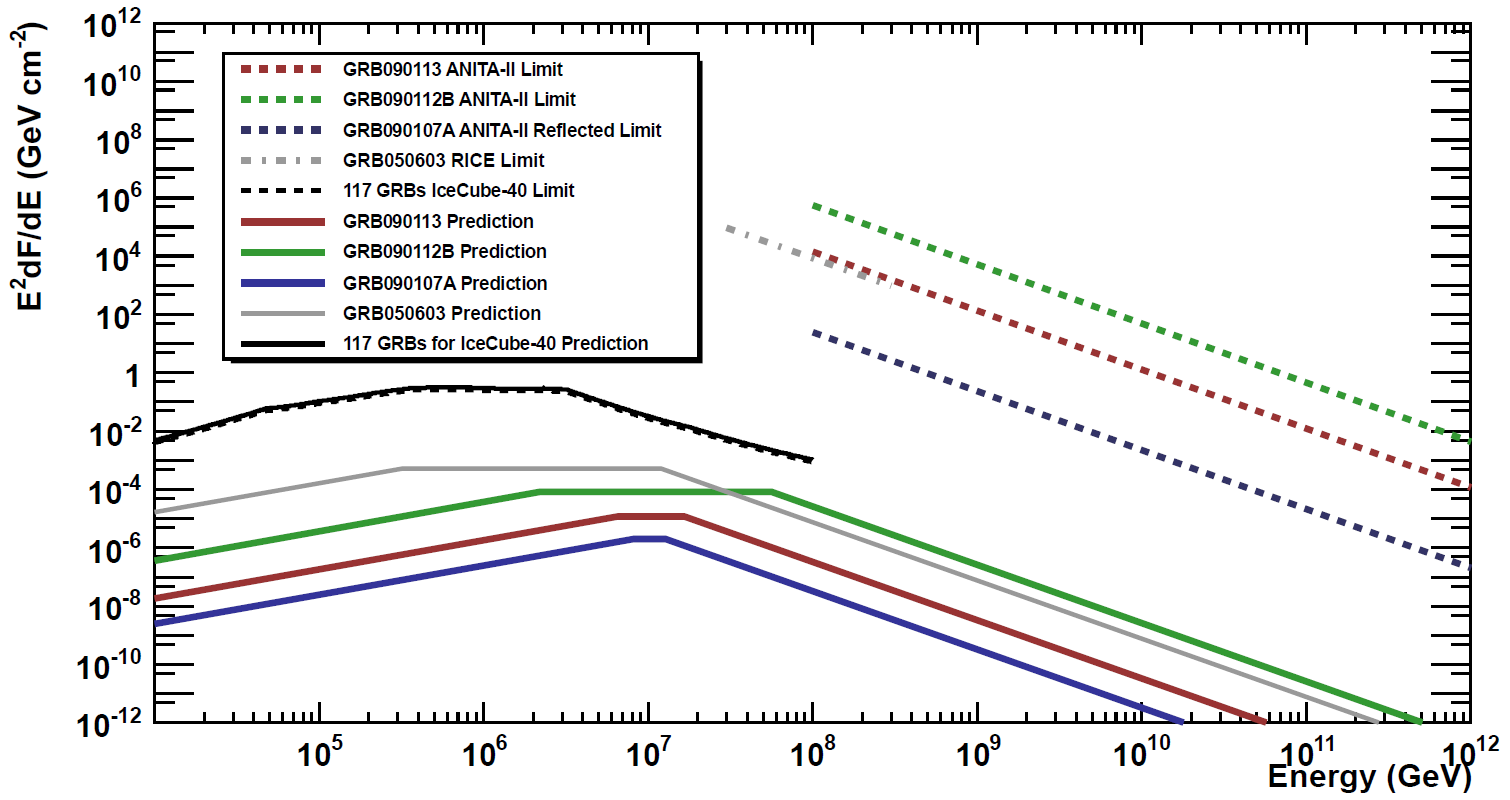
\includegraphics[width=1.0\textwidth]{figures/anitaresult.PNG}
\caption{Figure from ANITA publication on a GRB search~\cite{anita_grb}. The two best ``direct" limits by \gls{anita} on the UHE neutrino fluence from the blind analysis are from \gls{grb} 090113 and \gls{grb} 090112B. These are shown with red and green dashed lines respectively. The ``reflected" limit is from \gls{grb} 090107A, shown with a blue dashed line. RICE (Besson \textit{et al}. 2007) and IceCube (2012) \cite{IC2012} limits are also shown. The IceCube limit is an aggregate limit based on 117 individual \gls{grb}s, and is based on a fluence prediction from Guetta \textit{et al}. (2004) \cite{guetta,anita_grb}.}
\label{anitaresult}
\end{figure}

No events were found in the prompt emission or the precursor windows of the observed bursts. A limit was set for each burst individually on the prompt \gls{uhe} neutrino fluence using a Feldman-Cousins 90\% confidence interval, the duration of the burst, and the acceptance calculated using a Monte Carlo simulation. For each \gls{grb}, the Monte Carlo was configured to simulate a point source at the location of the burst, fixed \gls{anita} at the location of the payload during the burst, and assumed an input $E^{-4}$ (for UHE) spectrum.

None of the 26 \gls{grb}s during the flight had a payload elevation angle between $-25^{\circ}$ and the horizon which is where the authors claimed \gls{anita} has the best chance of seeing direct neutrino events. Of the 12 \gls{grbs} observed during quiet time, the most promising direct observation geometry was thought to be from \gls{grb} $090113$ at an elevation angle of $-25.7^{\circ}$ although this still suffered from poor geometry. \gls{anita} placed a 90\% confidence level limit on the $E^{-4}$ prompt neutrino fluence for energies $10^{17} \, \mathrm{eV} < E < 10^{21} \, \mathrm{eV}$ of $E^{4} \, \Phi = 1.5 \times 10^{20} \, \mathrm{ GeV^{3} \, cm^{-2}}$ from \gls{grb} $090113$. 

Figure~\ref{anitaresult} shows the three best limits placed by \gls{anita} in this \gls{grb}-coincident search. The red and green dashed lines are the ``direct" limits and the blue dashed line is the ``reflected" limit. Note that the reflected limit is the best limit. The ``reflected" limit comes from a \gls{grb} with an elevation angle of $0.5^{\circ}$, that is, a neutrino from this \gls{grb} would be down-going. It seems the authors stipulated that a down-going neutrino can only be seen by reflection off of an ice-shelf. Since this GRB was at a time when the payload was flying over the Ross Ice Shelf, the authors considered this \gls{grb} even though its background was not thermal-like. However, the authors did not consider \gls{grb} 090111 which had an elevation angle of $1.7^{\circ}$ because the payload was not over the Ross Ice Shelf when this \gls{grb} took place. Finally, note that the green dashed-line limit is almost two orders of magnitude worse than the red dashed-line limit. Both \gls{grbs} corresponding to these two limits had poor geometry or elevation angle of $-25.7^{\circ}$ (red dashed-line) and $-26.8^{\circ}$ (green dashed-line), respectively. 
Therefore, it is not surprising that these limits are not very tight. It is interesting, however, that a difference in elevation angle of just a degree can potentially make the limit much worse.

\subsection{First GRB search by ARA (2015)}

In 2015, the ARA collaboration presented an UHE \gls{grb} neutrino fluence limit from 57 selected \gls{grbs} and the first limit on the UHE \gls{grb} quasi-diffuse neutrino flux for energies $10^{16} \, \mathrm{ eV}$ to $10^{19} \, \mathrm{ eV}$ \cite{araproto} using data collected by ARA in prototype form (ARA Testbed) \cite{arahardware}. See Figure \ref{arafluence} and Figure \ref{araquasiflux}.

The quasi-diffuse flux is an estimation of the average \gls{grb} flux calculated from a statistically representative set of \gls{grb}s and is useful in comparing limits between experiments that observe different sets of bursts.

Predictions for \gls{grb} neutrino fluences were calculated using NeuCosmA~\cite{neucosma1,neucosma2}. For all \gls{grbs}, the bulk Lorentz factor of the fireball $\Gamma$ was assumed to be 316 and the baryonic loading (ratio of fractional proton energy to fractional electron energy) was assumed to be 10. As ARA is sensitive to all neutrino flavors, neutrino fluence predictions for all three flavors were obtained from NeuCosmA with 1:1:1 flavor ratio assumption. AraSim, a Monte-Carlo simulation software package used within the ARA collaboration, was used to simulate neutrino signals as they would be observed by the detector. It simulates the full chain of neutrino events such as the neutrino's path through the Earth, radio Cherenkov emission, the path and response of the emitted signal in the ice, and the trigger and data acquisition mechanisms of the detector \cite{araproto}. 

Among 589 \gls{grbs} monitored by the Gamma Ray Coordinate Network (GCN) catalog from January 2011 to December 2012 over the entire sky, 57 \gls{grbs} were selected for analysis because they occurred during a period of low anthropogenic background and high stability of the station and fell within the geometric acceptance.

Drawing on the blinding technique of analysis carried out by the \gls{anita} \gls{grb} neutrino search, the ARA collaboration performed a blind analysis with two un-blinding steps. ARA, too, used the 55 minutes before 1 hour and the 55 minutes after 5 minutes of a burst to study the background for each burst. For an extra step of caution, initially, only 10\% of the total 110 minutes of data temporally close to the 10 minutes of signal region was used to get cuts. Then, the remaining 90\% was used to get cuts and it was checked that these cuts were consistent with the ones from the initial 10\%. Only after this two-step method of getting analysis cuts was the analyzer unblinded to the signal region.
In the search for UHE neutrinos from 57 \gls{grbs} in \cite{araproto}, 0 events were observed, which was consistent with 0.11 expected background events.

\begin{figure}
\centering
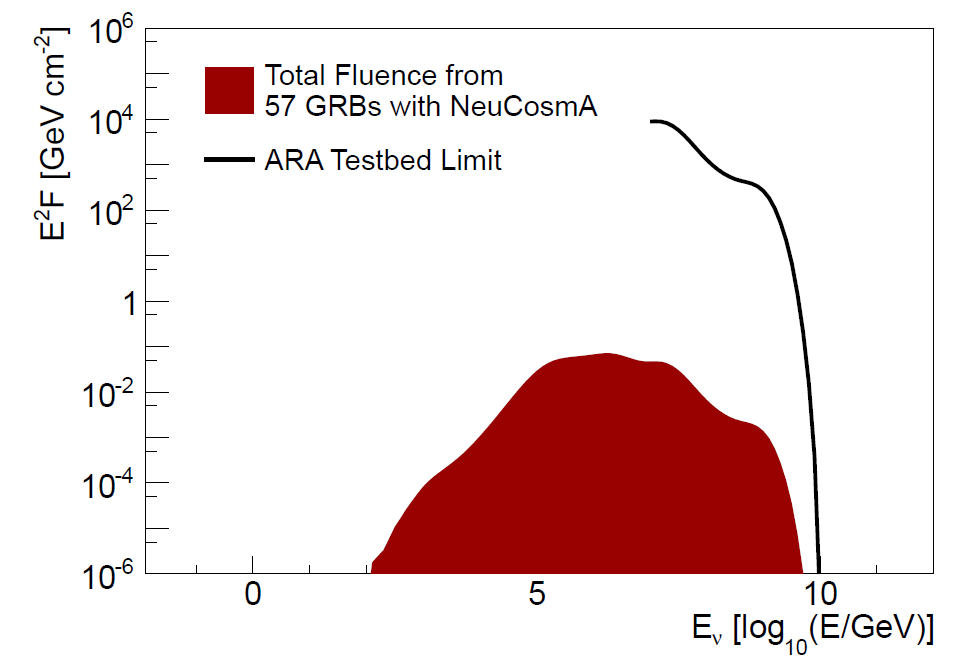
\includegraphics[width=.8\textwidth]{figures/ara_limit.png}
\caption{Figure from ARA publication on a GRB search~\cite{araproto}.
The limit on the UHE \gls{grb} neutrino fluence from 57 \gls{grbs} used for ARA analysis. Total fluence from NeuCosmA for the 57 \gls{grbs} is shown with a red shaded area and the limit from the ARA Testbed above $10^{16}$ eV is shown with a black solid curve.}
\label{arafluence}
\centering
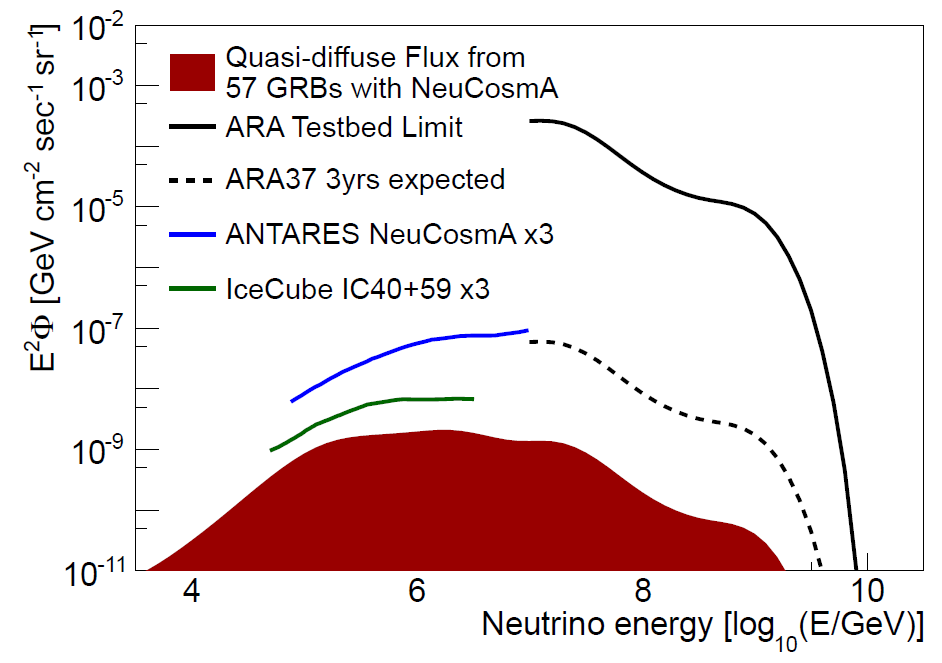
\includegraphics[width=.8\textwidth]{figures/ara_quasi_diffuse_limits.png}
\caption{Figure from ARA publication on a GRB search~\cite{araproto}. 
The inferred quasi-diffuse all flavor flux limit from the selected 57 \gls{grbs}. IceCube and ANTARES limits are from \cite{IC2012} and \cite{antaresmuon}, respectively.}
\label{araquasiflux}
\end{figure}

\section{Current theories}

The flux of neutrinos emitted during the afterglow period of \gls{grbs} is most interesting to \gls{anita}. This is because it is during the afterglow period of \gls{grbs} that \gls{uhe} neutrinos with energy $>10^{18}\,\mbox{eV}$ are predicted. 
Some of the earliest calculations for afterglow neutrino fluxes came from Waxman and Bahcall, for example, in~\cite{afterglows}.  
Since then, several other models have been developed, such as, by Kohta in~\cite{kohta}. 

The afterglow neutrino spectrum depends on the matter profile of the interstellar medium. This makes sense as the afterglow emission is due to collisions of the \gls{grb} plasma shells with the external material surrounding it, that is, the interstellar medium. Figure~\ref{mauricio} shows a plot made by \gls{grb} theorist Mauricio Bustamante. This shows the diffuse afterglow neutrino spectrum for two choices of matter profile and for the case where the afterglow is due to late internal collisions. 

Figure~\ref{mauricio} helps to summarize why \gls{anita} should include \gls{grb} afterglows in a \gls{grb} neutrino search. 
Late internal collisions are a variation of the prompt phase collisions, shown in solid pink in Figure~\ref{mauricio}. As can be seen from the horizontal axis representing energy in units of GeV, this late prompt phase model produces a neutrino flux only upto about $>10^{9}\,\mbox{GeV}$ or $10^{18}\,\mbox{eV}$. If a late prompt model cannot produce neutrinos above $10^{18}\,\mbox{eV}$, a regular prompt model is even less expected to do so. In contrast, the afterglow models shown in solid green and blue in Figure~\ref{mauricio} go above $10^{18}\,\mbox{eV}$. This is where \gls{anita} starts to become sensitive. Therefore, in order to detect neutrinos from \gls{grbs} with \gls{anita} it would be best to include afterglow periods. 

\begin{figure}
\centering
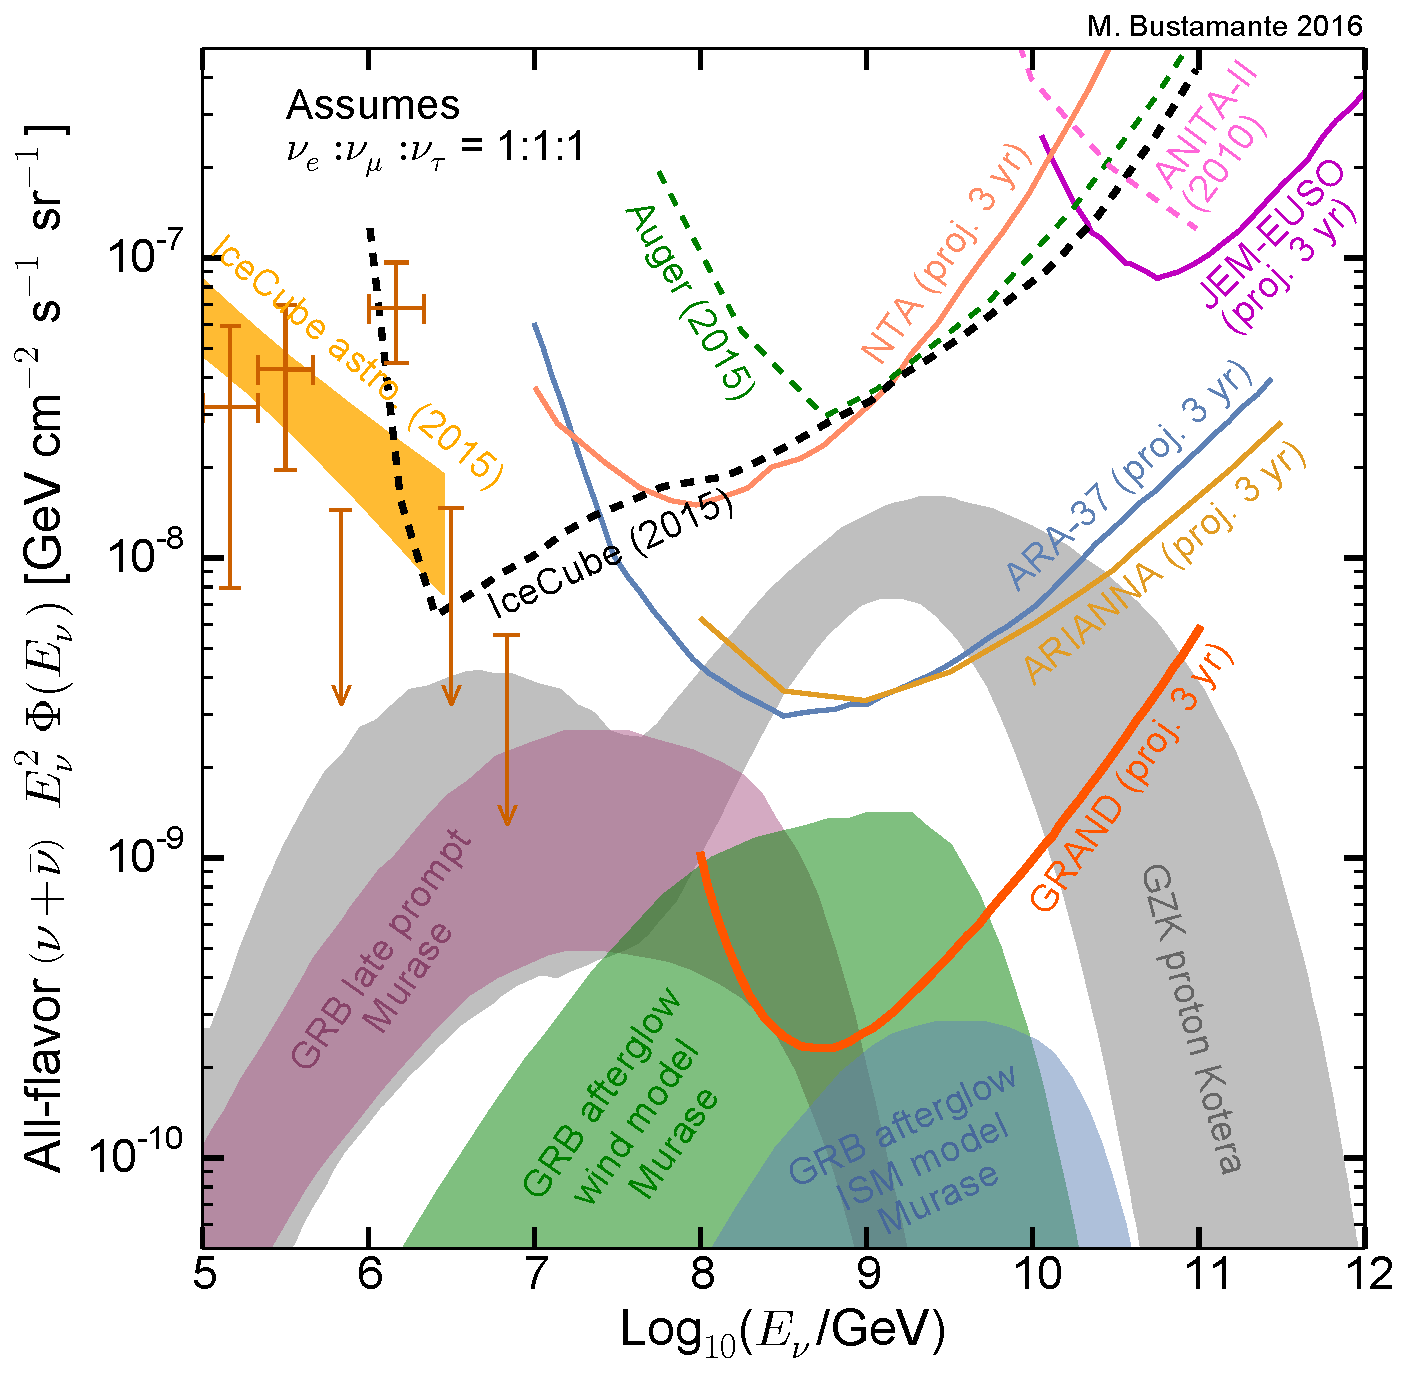
\includegraphics[width=1.0\textwidth]{figures/mauricio_plot.pdf}
\caption{Figure by Mauricio Bustamante, unpublished. This shows different models for neutrino spectra.}
\label{mauricio}
\end{figure}